\documentclass[fontsize=8pt]{scrartcl}
\usepackage[T1]{fontenc}
\usepackage[utf8]{inputenc}
\usepackage{multicol} % for multicols environment
\usepackage{mathtools} % loads amsmath, for math environments etc
\usepackage{geometry} % for defining margins etc
\usepackage{tabularx}% http://ctan.org/pkg/tabularx
\usepackage{makecell}
\usepackage{cancel}
\usepackage{float}
\usepackage{xcolor}
\usepackage{amsmath}
\usepackage{tikz}
\usetikzlibrary{calc}
\renewcommand\tabularxcolumn[1]{m{#1}}
\geometry{
 margin=0.7cm
}

\newcommand{\mysection}[1]{
    \setlength\fboxsep{4pt} %% spacing around box contents
    \section*{\colorbox{black}{\makebox[\linewidth][l]{\color{white}#1\hfill}}}
}

\definecolor{light-gray}{gray}{0.95}
% put color to \boxed math command
\newcommand*{\boxcolor}{light-gray}
\makeatletter
\renewcommand{\boxed}[1]{
    \textcolor{\boxcolor}{%
        \tikz[baseline={([yshift=-1ex]current bounding box.center)}]
        \node [fill=light-gray, minimum width=1ex,draw]
        {\normalcolor\m@th$\displaystyle#1$};
    }
}
 \makeatother
\allowdisplaybreaks % allow environments like gather and align to break across columns/pages
\begin{document}

\begin{multicols*}{2}
\mysection{PIANI DI CAMPIONAMENTO PER VARIABILI}
\begin{align*}
n&=\left(\frac{Z_\alpha+Z_\beta}{Z_{AQL}+Z_{LTPD}}\right)^2\overbracket{\boxed{\left(1+\frac{K^2}{2}\right)}}^{\text{se \(\sigma\) non nota}}\\
K&=\frac{-\left(Z_\alpha Z_{LPTD} + Z_\beta Z_{AQL}\right)}{Z_\alpha+z_\beta}\\
Z_{LSI} &= \frac{\overline{x}-LSI}{\sigma}\\
P_a &= \phi \Bigg(\frac{\sqrt{n}(K + Z_p)}{{\underbracket{\boxed{\sqrt{1+\frac{k^2}{2}}}}_{\text{se \(\sigma\) non nota}}}}\Bigg)
\end{align*}

\subsection*{Metodo K}
\begin{equation*}
    \boxed{ Z_{LSI} \geq K } 
\end{equation*}

\subsection*{Metodo M}
\begin{align*}
Q_{LSI} &= Z_{LSI}\sqrt{\frac{n}{n-1}} \\
\widehat{p} &=  \phi \left(-Q_{LSI}\right)\\
M &= \phi\left(-K\sqrt{\frac{n}{n-1}}\right)
\end{align*}
\begin{equation*}
    \boxed{\widehat{p} < M}
\end{equation*}
\vfill\null
\columnbreak

\mysection{PIANI DI CAMPIONAMENTO PER ATTRIBUTI}
\begin{center}
    \begin{tabularx}{\linewidth}{r X}
        \(\alpha\) & Rischio del fornitore\\
        \(\beta\) & Rischio del committente\\
        \(AQL\) & Valore limite di difettositá al di sopra del quale il fornitore è disposto a vedersi rifiutare il lotto con rischio \(\alpha\)\\
        \(LTPD\) & Valore limite di difettositá al di sotto del quale il committente accetta il lotto con rischio \(\beta\)\\
        \(AOQ\) & difettositá media in uscita\\
        \(AOQL\) & difettositá massima in uscita\\
        \(ATI\) & Average Total Inspection, numero medio di controlli totali\\
    \end{tabularx}
\end{center}
\begin{align*}
    &\begin{cases}
        1-\alpha = \sum_{i=0}^c\binom{n}{i}AQL^i(1-AQL)^{n-i}\\
        \beta = \sum_{i=0}^c\binom{n}{i}LTPD^i(1-LTPD)^{n-i}\\
    \end{cases}\\
    P_a &= \sum_{i=1}^c\binom{n}{i}p^i(1-p)^{n-i}\\
\end{align*}

\subsection*{Piano Singolo}

\begin{center}
    \begin{tabular}{ |c|c|c| }
        \hline
              & sostituzione & no sostituzione\\  \hline
        ATI & \multicolumn{2}{c|}{\(P_an+(1-P_a)N\)}\\  \hline
        AOQ & \(\frac{P_a p(N-n)}{N}\) & \(\frac{P_a p(N-n)}{N - p(ATI)}\)  \\ \hline
        AOQL & \multicolumn{2}{c|}{\( \frac{\partial AOQ}{\partial p}=0 \rightarrow \text{calcolato con \(p_{max}\)}\)}\\ \hline  
    \end{tabular}
\end{center}

\subsection*{Piano Doppio}
\begin{center}
    \begin{tabular}{|c|c|c|}
        \hline
               & sostituzione & no sostituzione\\  \hline
          ATI  & \multicolumn{2}{c|}{\( n_1P_I+(n_1+n_2)P_{II}+N(1-P_I-P_{II}) \)}\\  \hline
          AOQ  & \( \frac{P_Ip(N-n_1)+P_{II}p(N-n_1-n_2)}{N}\) & \( \frac{P_Ip(N-n_1)+P_{II}p(N-n_1-n_2)}{N - p(ATI)}\) \\ \hline
          AOQL & \multicolumn{2}{c|}{\( \frac{\partial AOQ}{\partial p}=0 \rightarrow \text{calcolato con \(p_{max}\)}\)}\\ \hline
          ASN  &\multicolumn{2}{c|}{\( n_1P_I+(n_1+n_2)(1-P_I) \)}\\ 
        \hline  
    \end{tabular}
\end{center}

\subsection*{Piano A Catena}
\begin{center}
    \begin{tabularx}{\linewidth}{r X}
        \(P(0,n)\) & Probabilitá di avere 1 difettoso\\
        \(P(1,n)\) & Probabilitá di avere 0 difettosi\\
    \end{tabularx}
\end{center}
\begin{align*}
    P_a = P(0,n) + P(1,n)P(0,n)^i
\end{align*}

\subsection*{Errori di ispezione}
\begin{align*}
    p_e &= (1-p)e_1+p(1-e_2)\\
    p_a(p_e)&=p_{eA}-ATI'=\\
            &=\sum \left[n+(1-p_{eA})(N-n)\right]p_{eA}^i=\\
            &=\frac{n+(1-p_{eA})(N-n)}{1-p_{eA}}
\end{align*}
\vfill\null
\columnbreak

\mysection{CARTE DI CONTROLLO PER VARIABILI}

\subsection*{Carta \(\mathbf{X-R}\)}

\begin{align*}
    \sigma_P&=\frac{\overline{R}}{d_2}\\
    \mu_P&=\overline{\overline{X}}\\
    \sigma_X&=\frac{\sigma_P}{\sqrt{n}}\\
    \mu_X&=\mu_P\\
    \sigma_R&=\sigma_Pd_3\\
    \mu_R&=\overline{R}\\
    LC_X&=\mu_X\pm L\sigma_X\\
    LC_R&=\mu_R\pm L\sigma_R\\
\end{align*}

\subsection*{Carta \(\mathbf{X-S}\)}

\begin{align*}
    \sigma_P&=\frac{S}{c_4}\\
    \mu_P&=\overline{\overline{X}}\\
    \sigma_X&=\frac{\sigma_P}{\sqrt{n}}\\
    \mu_X&=\mu_P\\
    \sigma_S&=\sqrt{1-c_4^2}\sigma_P\\
    \mu_S&=\overline{S}\\
    LC_X&=\mu_X\pm L\sigma_X\\
    LC_S&=\mu_S\pm L\sigma_S\\
\end{align*}

\subsection*{Carta \(\mathbf{X-R_{mobile}}\)}

\begin{align*}
    \sigma_P&=\frac{\overline{R}}{d_2}\\
    \mu_P&=\overline{\overline{X}}\\
    \sigma_X&=\frac{\sigma_P}{\sqrt{n}}\\
    \mu_X&=\mu_P\\
    \sigma_R&=\sigma_Pd_3\\
    \mu_R&=\overline{R}\\
    LC_X&=\mu_X\pm L\sigma_X\\
    LC_R&=\mu_R\pm L\sigma_R\\
\end{align*}

\begin{center}
    \begin{tabularx}{\linewidth}{r X}
        \(TN \)       & \(6\sigma_p\)\\
        \(\beta\) & Probabilitá di \textit{non} identificare un fuori controllo\\
        \(1-\beta^i\) & Probabilitá di identificare un fuori controllo entro l'i-esimo campionamento\\
        \(ARL\) & \(\frac{1}{1-\beta}\) numero medio di campioni prima di rilevare un fuori controllo\\
        \(ARL_0\) & \(\frac{1}{\alpha}\) ogni quanti campioni mi aspetto un falso fuori controllo\\
        \(ATS\) & \(ARL \times h\) tempo che passa prima del verificarsi di un fuori controllo\\
    \end{tabularx}
\end{center}
\vfill\null
\columnbreak

\mysection{CARTE DI CONTROLLO PER ATTRIBUTI}
\subsection*{Carta \(\mathbf{p}\)}
Binomiale
\begin{align*}
    \widehat{p} &= \frac{difettosi}{n}\\
    \overline{p}&=\frac{\sum \widehat{p}}{k}\\
    LC &= \overline{p} \pm L\sqrt{\frac{\overline{p}(1-\overline{p})}{n}}   
\end{align*}

\subsection*{Carta \(\mathbf{np}\)}
Binomiale
\begin{align*}
    LC &= n\overline{p} \pm L\sqrt{n\overline{p}(1-\overline{p})}
\end{align*}

\subsection*{Carta \(\mathbf{c}\)}
Poisson
\begin{align*}
    \overline{c}&=\frac{\sum Difetti}{k}\\
    LC &= \overline{c} \pm L\sqrt{\overline{c}}    
\end{align*}

\subsection*{Carta \(\mathbf{u}\)}
Poisson
\begin{align*}
    \widehat{u} &= \frac{difetti}{n}\\
    \overline{u}&=\frac{\sum \widehat{u}}{k}\\
    LC &= \overline{u} \pm L\sqrt{\frac{\overline{u}}{n}}    
\end{align*}

\mysection{DISTRIBUZIONI}

\begin{center}
    \begin{tabularx}{\linewidth}{c X}
        \(N\)             & Numero di elementi nel lotto\\
        \(m\)             & Numero di elementi difettosi nel lotto\\
        \(p=\frac{m}{N}\) & Percentuali di elementi difettosi nel lotto\\
        \(n\)             & Numerositá del campione estratto dal lotto\\
        \(c\)             & Numero massimo di elementi difettosi che possono essere presenti nel campione, numero di accettazione\\
        \(\lambda\)       & \(np\)\\
    \end{tabularx}
\end{center}

\subsection*{Ipergeometrica}
\begin{equation*}
    P_a(N,n,c,p)=\sum_{i=0}^c\frac{\binom{N-Np}{n-i} \binom{Np}{i}}{\binom{N}{n}}
\end{equation*}

\subsection*{Binomiale}
Carta \textit{p} e carta \textit{np}
\begin{equation*}
    P_a(n,c,p)=\sum_{i=0}^c\binom{n}{i}p^i(1-p)^{n-i}
\end{equation*}

\subsection*{Poisson}
Carta \textit{c} e carta \textit{u}
\begin{equation*}
    P_a(\lambda, c)=\sum_{i=0}^c\frac{\lambda^ie^{-\lambda}}{i!}
\end{equation*}

\subsection*{Approssimazioni}
\begin{center}
    \begin{tabular}{|c|c|}
        \hline
        \(N>10n\) & Ipergeometrica \(\rightarrow\) Binomiale\\\hline
        \(p>0.1\) & Binomiale \(\rightarrow\) Poisson\\\hline
        \(np \geq 5 \land  0.1<p<1\) & Binomiale \(\rightarrow\) Poisson\\\hline
        \(np > 5 \land np(1-p)>5\) & Binomiale \(\rightarrow\) Normale\\\hline
        \(\lambda > 10\) & Poisson \(\rightarrow\) Normale\\\hline
    \end{tabular}
\end{center}

\vfill\null
\columnbreak

\mysection{TEST MEDIA}
\begin{align*}
    \overline{x}&=\frac{\sum_ ix_i}{n}\\
    S&=\sqrt{\frac{(x_i-\overline{x})^2}{n-1}}
\end{align*}

\subsection*{\(\mathbf{\sigma}\) nota - Test Normale}

\subsubsection*{\(\mathbf{H_0:\mu=\mu_0}\)}

\begin{align*}
    z_{sp}&=\frac{\overline{x}-\mu_0}{\frac{\sigma}{\sqrt{n}}}
\end{align*}
\begin{equation*}
    \boxed{-z_{1-\frac{\alpha}{2}}\leq z_{sp} \leq z_{1-\frac{\alpha}{2}}}
\end{equation*}

\subsubsection*{\(\mathbf{H_0:\mu_1=\mu_2}\)}

\begin{align*}
    z_{sp}&=\frac{\overline{x_1}-\overline{x_2}}{\sqrt{\frac{\sigma_1^2}{n_1}+\frac{\sigma_2^2}{n_2}}}    
\end{align*}
\begin{equation*}
   \boxed{-z_{1-\frac{\alpha}{2}}\leq z_{sp} \leq z_{1-\frac{\alpha}{2}}}
\end{equation*}

\subsection*{\(\mathbf{\sigma}\) non nota, stimata da \(\mathbf{S}\) - Test t di student}

\subsubsection*{\(\mathbf{H_0:\mu=\mu_0}\)}
\begin{align*}
    T_{sp}&=\frac{\overline{x}-\mu_0}{\frac{S}{\sqrt{n}}}    
\end{align*}
\begin{equation*}
    \boxed{-t_{n-1,1-\frac{\alpha}{2}}\leq T_{sp} \leq t_{n-1,1-\frac{\alpha}{2}}}
\end{equation*}
\subsubsection*{\(\mathbf{H_0:\mu_1=\mu_2}\) ipotesi \(\mathbf{S_1=S_2}\)}
\begin{align*}
    S_{pool}&=\sqrt{\frac{(n_1-1)S_1^2+(n_2-1)S_2^2}{n_1+n_2-2}}\\
    T_{sp}&=\frac{\overline{x_1}-\overline{x_2}}{\frac{S_{pool}}{\sqrt{n_1+n_2}}}    
\end{align*}
\begin{equation*}
    \boxed{-t_{n_1+n_2-2,1-\frac{\alpha}{2}}\leq T_{sp} \leq t_{n_1+n_2-2,1-\frac{\alpha}{2}}}
\end{equation*}
\subsubsection*{\(\mathbf{H_0:\mu_1=\mu_2}\) ipotesi \(\mathbf{S_1\neq S_2}\)}
\begin{align*}
    \overline{n}&=\frac{\frac{S_1^2}{n_1}+\frac{S_2^2}{n_2}}{\frac{(\frac{S_1^2}{n_1})^2}{n_1-1}+\frac{(\frac{S_2^2}{n_2})^2}{n_2-1}} \\
    T_{sp}&=\frac{\overline{x_1}-\overline{x_2}}{\sqrt{\frac{S_1^2}{n_1}+\frac{S_2^2}{n_2}}}    
\end{align*}
\begin{equation*}
    \boxed{-t_{n_1+n_2-2,1-\frac{\alpha}{2}}\leq T_{sp} \leq t_{n_1+n_2-2,1-\frac{\alpha}{2}}}
\end{equation*}
\vfill\null
\columnbreak

\mysection{TEST VARIANZA}

\subsection*{Test \(\mathbf{\chi^2}\)}

\subsubsection*{\(\mathbf{H_0:\sigma^2=\sigma^2_0}\)}
\begin{align*}
    \chi^2_{sp}&=\frac{(n-1)S^2}{\sigma_0^2}    
\end{align*}
\begin{equation*}
    \boxed{\chi^2_{n-1;\frac{\alpha}{2}}\leq \chi^2_{sp} \leq \chi^2_{n-1;1-\frac{\alpha}{2}}}
\end{equation*}

\subsection*{Test Fisher}

\subsubsection*{\(\mathbf{H_0:\sigma^2_1=\sigma^2_2}\)}
\begin{align*}
    F_{sp} &= \frac{S_1^2}{S_2^2}
\end{align*}
\begin{equation*}
    \boxed{F_{n_1-1;n_2-1;\frac{\alpha}{2}}\leq F_{sp}\leq F_{n_1-1;n_2-1;1-\frac{\alpha}{2}}}
\end{equation*}
\begin{equation*}
    F_{A;B;1-\alpha}=\frac{1}{F_{B;A;\alpha}}
\end{equation*}

\vfill\null
\columnbreak

\mysection{DIFETTOSITÁ REALE E APPARENTE}

\begin{align*}
    p_{reale} &= p_{apparente} - \text{falsi difettosi} + \text{falsi buoni}\\
              &= p_{apparente} - (1-p_{reale})\alpha + p_{reale}\beta
\end{align*}

\mysection{METODI DI VOTO}

\begin{center}
    \begin{tabular}{|l|c|c|c|c|}
        \hline
                        & \(\alpha\) & \(\beta\) & \(\gamma\) & \(\rho\)\\\hline
        produzione \(I_1\) & 360 & 362 & 359 & 358 \\\hline
        difetti \(I_2\) & 35 & 32 & 36 & 40 \\\hline
        difettositá \(I_3\) & 4\% & 5.5\% & 4.5\% & 5\% \\\hline
    \end{tabular}
\end{center}

\subsection*{Metodo Best of the best}

\begin{align*}
    I_1 = \gamma > \beta > \alpha > \rho\\
    I_2 = \beta > \alpha > \gamma > \rho\\
    I_3 = \alpha > \gamma > \rho > \beta
\end{align*}

\subsection*{Metodo Borda}

\begin{center}
    \begin{tabular}{c c c c c}
                    & \(\alpha\)  & \(\beta\) & \(\gamma\)& \(\rho\)\\
            \(I_1\) & 2°  & 1° & 3° & 4°\\
            \(I_2\) & 2° & 1° & 3° & 4°\\
            \(I_3\) & 1° & 4° & 2° & 3°\\\hline
            \(\sum\)& 5 & 6 & 8 & 11
    \end{tabular}
    \begin{equation*}
        \text{bottom to top: } \alpha > \beta > \gamma > \rho
    \end{equation*}
\end{center}

\subsection*{Metodo Condorcet}

\begin{center}
    \begin{tabular}{c c c c c|c}
                    & \(\alpha\)  & \(\beta\) & \(\gamma\)& \(\rho\) & min\\
            \(\alpha\)  & - & 1 & 3 & 3 & 1\\
            \(\beta\)   & 2 & - & 2 & 2 & 2\\
            \(\gamma\)  & 0 & 1 & - & 3 & 0\\
            \(\rho\)    & 0 & 1 & 0 & - & 0\\
    \end{tabular}
    \begin{equation*}
        \text{top to bottom: } \beta > \alpha > \gamma \sim \rho
    \end{equation*}
\end{center}

\mysection{SCALE}
\begin{center}
    \begin{tabularx}{\linewidth}{|c|c|X|}
        \hline
       TRASFORMAZIONI & TIPOLOGIA & \multicolumn{1}{c|}{ESEMPI} \\\hline
       \(\phi (x)=x\) & Assoluta & conteggi\\\hline
       \makecell{Similitudine \\ \(\phi (x)=\alpha x\)} & Rapporto & massa, temperatura in kelvin, tempo, suono, lucentezza\\\hline
       \makecell{Lineare \\ \(\phi (x)=\alpha x + \beta\)} & Intervallo & temperatura, calendario\\\hline
       \(x \geq y \Leftrightarrow \phi(x)\geq\phi(y)\) & Ordinale & classifiche, qualitá dell'aria, durezza\\\hline
       Qualsiasi a uno a uno & Nominale & maglie giocatori, colore occhi\\\hline
    \end{tabularx}
\end{center}

\subsection*{Compensazione}
\begin{align*}
    OEE &= A\times B\times C \rightarrow\\
   \rightarrow A&=\frac{OEE}{B\times C} \rightarrow\\
   \rightarrow \frac{\partial A}{\partial B}&=\frac{OEE}{B^2\times C} \rightarrow\\
   \rightarrow \partial A&=\frac{A\times \cancel{B} \times C}{B^{\cancel{2}}\times C} \rightarrow\\
   \rightarrow \Delta A&=-A\frac{\Delta B}{B} \rightarrow\\
\end{align*}

\subsection*{Monotonia}
\begin{align*}
    \frac{\partial I}{\partial A} &\geq 0
\end{align*}
\vfill\null
\columnbreak

\mysection{INDICI DI CAPACITÁ}

\subsection*{Indice \(\mathbf{C_p}\)}

\begin{align*}
    C_p&=\frac{LSS-LSI}{6\sigma_p} \boxed{> 1.33}
\end{align*}

\subsection*{Indice \(\mathbf{C_p}\)}

\begin{align*}
    C_{pi}&=\frac{\mu-LSI}{3\sigma_p} \boxed{> 1.25}\\
    C_{ps}&=\frac{LSS-\mu}{3\sigma_p} \boxed{> 1.25}\\
    C_{pk}&=min(C_{pi},C_{ps}) \boxed{> 1.33}
\end{align*}

\mysection{GEOMETRIA}

\subsection*{Trigonometria}

\begin{minipage}[m]{.45\linewidth}
    \begin{figure}[H]
        \centering
        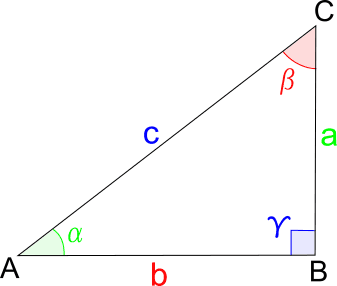
\includegraphics[width=.5\linewidth]{images/triangolo_rettangolo.png}
    \end{figure}
\end{minipage}
\begin{minipage}[m]{.45\linewidth}
    \begin{align*}
        a &= c\sin(\alpha)\\
        a &= c\cos{\beta}\\
        b &= c\sin{\beta}\\
        b &= c\cos{\alpha}
    \end{align*}
\end{minipage}

\subsection*{Grandezze}

\begin{center}
    \begin{tabular}{|r|c|}
        \hline
        Circonferenza: & \(2\pi r\)\\\hline
        Cerchio: & \(\pi r^2\)\\\hline
        Superficie sfera: & \(4\pi r^2\)\\\hline
        Volume sfera: & \(\frac{4}{3}\pi r^3\)\\\hline
    \end{tabular}
\end{center}

\mysection{ELETTROTECNICA}

\subsection*{Parallelo}

\begin{minipage}[m]{.45\linewidth}
    \begin{figure}[H]
        \centering
        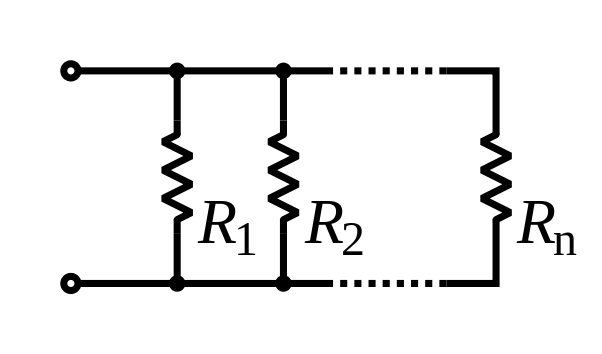
\includegraphics[width=.8\linewidth]{images/parallelo.png}
    \end{figure}
\end{minipage}
\begin{minipage}[m]{.45\linewidth}
    \begin{equation*}
        R_{eq}=\left( \frac{1}{R_1}+\frac{1}{R_2} \right)^{-1} = \frac{R_1R_2}{R_1+R_2}
    \end{equation*}
\end{minipage}

\subsection*{Serie}

\begin{minipage}[m]{.45\linewidth}
    \begin{figure}[H]
        \centering
        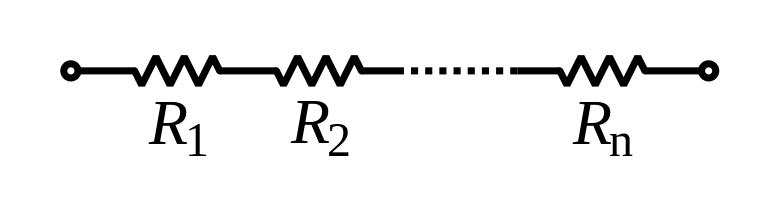
\includegraphics[width=.8\linewidth]{images/serie.png}
    \end{figure}
\end{minipage}
\begin{minipage}[m]{.45\linewidth}
    \begin{equation*}
        R_{eq}=R_1+R_2
    \end{equation*}
\end{minipage}

\subsection*{Partitore di Corrente}

\begin{minipage}[m]{.45\linewidth}
    \begin{figure}[H]
        \centering
        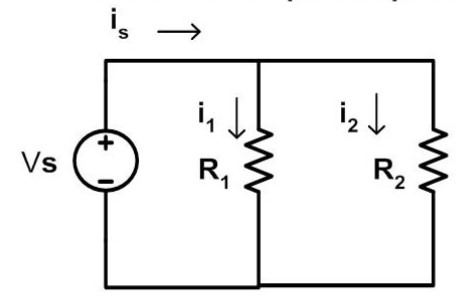
\includegraphics[width=.8\linewidth]{images/partitore_corrente.jpg}
    \end{figure}
\end{minipage}
\begin{minipage}[m]{.45\linewidth}
    \begin{align*}
        i_1 &= i_s\frac{R_2}{R_1+R_2}\\
        i_2 &= i_s\frac{R_1}{R_1+R_2}
    \end{align*}
\end{minipage}

\subsection*{Partitore di Tensione}

\begin{minipage}[m]{.45\linewidth}
    \begin{figure}[H]
        \centering
        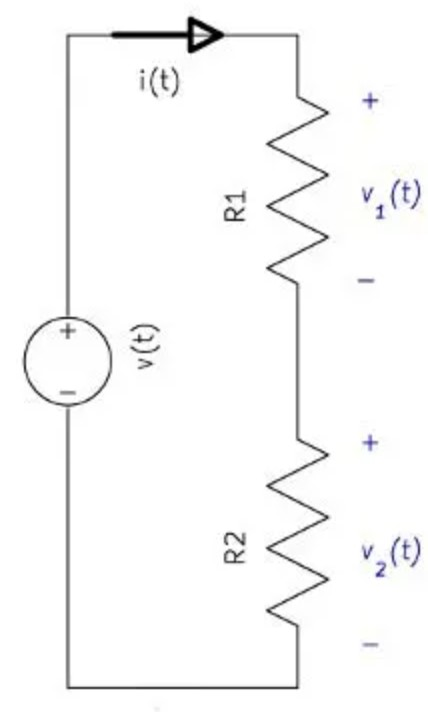
\includegraphics[width=.4\linewidth]{images/partitore_tensione.jpg}
    \end{figure}
\end{minipage}
\begin{minipage}[m]{.45\linewidth}
    \begin{align*}
        V_1 &= V_s\frac{R_1}{R_1+R_2}\\
        V_2 &= V_s\frac{R_2}{R_1+R_2}
    \end{align*}
\end{minipage}

\end{multicols*}
\end{document}